\documentclass[12pt]{report}
\usepackage[utf8]{inputenc}
\usepackage[T1]{fontenc}
\usepackage{pdfpages, indentfirst, extarrows, amsfonts, amssymb, amsmath, amsthm, mathrsfs, mathtools, esvect, abstract, color, appendix, centernot, relsize, accents, multicol, listings, natbib, indentfirst, graphicx, hyperref, lipsum, xcolor, tikz, siunitx, setspace, fancyhdr}
\usepackage[most]{tcolorbox}
\usepackage[brazil]{babel}
\usepackage[nottoc,numbib]{tocbibind}
\usepackage[justification=centering]{subfig}
\usepackage[font=small,labelfont=bf]{caption}
\usepackage[shortlabels]{enumitem}
\usepackage[explicit]{titlesec}
\usepackage[Conny]{fncychap}
%Options: Sonny, Lenny, Glenn, Conny, Rejne, Bjarne, Bjornstrup

\hypersetup{
    colorlinks=true,
    linktoc=all,
    linkcolor=blue,
    urlcolor=red,
    % pdftitle={How to write a thesis},
}
\def\mydate{\today}
\onehalfspacing %setspace
\graphicspath{ {./img/} }

% \pagestyle{fancy}
% \lhead{Trefor's awesome LaTeX guide}
% \rhead{Sponsored by Overleaf!}
% \cfoot{Page \thepage\ of \pageref{LastPage}}
% \setlength{\headheight}{14.49998pt}


\newcommand{\corText}[2]{{\color{#1} #2}}
\newcommand{\colorBoxSimples}[1]{\begin{tcolorbox}#1\end{tcolorbox}}
\newcommand{\colorBoxTitle}[2]{\begin{tcolorbox}[colback=red!5!white,colframe=red!50!black,title=#1]
        #2\end{tcolorbox}}
\newcommand{\inLine}[1]{$#1$}
\newcommand{\ela}[1]{\begin{equation*}\mathlarger{\begin{aligned}#1\end{aligned}}\end{equation*}}
\newcommand{\ea}[1]{\begin{equation*}\begin{aligned}#1\end{aligned}\end{equation*}}
\newcommand{\eal}[2]{\begin{equation}\tag{#1}\begin{aligned}#2\end{aligned}\end{equation}}
\newcommand{\elal}[2]{\begin{equation}\tag{#1}\mathlarger{\begin{aligned}#2\end{aligned}}\end{equation}}
\newcommand{\elg}[1]{\begin{equation*}\mathlarger{\begin{gathered}#1\end{gathered}}\end{equation*}}
\newcommand{\elgl}[2]{\begin{equation}\tag{#1}\mathlarger{\begin{gathered}#2\end{gathered}}\end{equation}}
\newcommand{\es}[1]{\begin{equation*}\begin{split}#1\end{split}\end{equation*}}
\newcommand{\esl}[2]{\begin{equation}\tag{#1}\begin{split}#2\end{split}\end{equation}}
\newcommand{\els}[1]{\begin{equation*}\mathlarger{\begin{split}#1\end{split}}\end{equation*}}
\newcommand{\elsl}[2]{\begin{equation}\tag{#1}\mathlarger{\begin{split}#2\end{split}}\end{equation}}
\newcommand{\matriz}[2]{\begin{#1matrix}#2\end{#1matrix}}
\newcommand{\overeq}[1]{\stackrel{\mathclap{\normalfont\mbox{#1}}}{\mathlarger{\mathlarger{\mathlarger{\mathlarger{=}}}}}}
\newcommand{\overs}[2]{\stackrel{\mathclap{\normalfont\mbox{#2}}}{\mathlarger{\mathlarger{#1}}}}
\newcommand{\overiff}[1]{\xLongleftrightarrow{#1}}
\newcommand{\overimplies}[1]{\xRightarrow{#1}}
\newcommand{\bs}[1]{\boldsymbol {#1}}
\newcommand{\rfig}[1]{Figura \ref{fig:#1}}
\newcommand{\genvs}[1]{\langle #1 \rangle}
\newcommand{\ip}[2]{\left\langle  #1 , #2  \right\rangle}
\newcommand{\der}[2]{\frac{\mathrm{d}#1}{\mathrm{d}#2}}
\newcommand{\pder}[2]{\frac{\partial#1}{\partial#2}}
\newcommand{\parenteses}[1]{\left(#1\right)}
\newcommand{\colchetes}[1]{\left[#1\right]}
\newcommand{\calcEm}[3]{\left.#1\right|^{#2}_{#3}}
\newcommand{\chaves}[1]{\left\{#1\right\}}
\newcommand{\function}[5]{#1:\begin{array}{rcl}#2&\longrightarrow & #3\\[-0.5mm]#4&\longmapsto &#5\end{array}}
\newcommand{\seq}[1]{\parenteses{#1}_{n\in\bN}}
\newcommand{\system}[1]{\left\{\begin{aligned}#1\end{aligned}\right.}
\newcommand{\st}[1]{| #1\rangle}
\newcommand{\ov}[1]{\overline{#1}}
\newcommand{\into}[1]{\stackrel{\circ}{#1}}
\newcommand{\integ}[4]{\int_{#1}^{#2}#3\,d#4}
\newcommand{\iinteg}[4]{\iint_{#1}^{#2}#3\,d#4}
\newcommand{\iiinteg}[4]{\iiint_{#1}^{#2}#3\,d#4}
\newcommand{\iiiinteg}[4]{\iiiint_{#1}^{#2}#3\,d#4}
\newcommand{\abs}[1]{\left| #1 \right|}
\newcommand{\norm}[1]{\left \lVert #1 \right \rVert}
\newcommand{\modulo}[1]{\left| #1 \right|}
\newcommand{\acl}[2]{\ov{#1}^{#2}}
\newcommand{\rest}[2]{{#1}_{\mkern 1mu \vrule height 2ex\mkern2mu {#2}}}

\newcommand{\boldText}[1]{\textbf{#1}}
\newcommand{\italic}[1]{\textit{#1}}
\newcommand{\linhaSep}{\begin{center}--------------------------------------------------------------------\end{center}}
\newcommand{\titulo}[1]{\begin{center}\boldText{\underline{#1}}\end{center}}
\newcommand{\itensBolas}[1]{\begin{itemize}#1\end{itemize}}
\newcommand{\itensLetras}[1]{\begin{enumerate}[label=\alph*)]#1\end{enumerate}}
\newcommand{\itensNumeros}[1]{\begin{enumerate}#1\end{enumerate}}


\newtheoremstyle{definition1}
{35pt} % Space above
{20pt} % Space below
{} % Body font
{} % Indent amount
{\bfseries} % Theorem head font
{.} % Punctuation after theorem head
{.5em} % Space after theorem head
{} % Theorem head spec (can be left empty, meaning `normal')

\newtheoremstyle{remark1}{25pt}{15pt}{}{}{\it}{.}{.5em}{}

\theoremstyle{definition1}
\newtheorem{teorema}{Teorema}[subsection]
\newtheorem{corolario}[teorema]{Corolário}
\newtheorem{lema1}{Lema}[subsection]
\newtheorem{proposicao}{Proposição}[subsection]
\newtheorem{definicao}{Definição}[subsection]
\newtheorem{exemplo}{Exemplo}[subsection]

\newtheorem*{teorema*}{Teorema}
\newtheorem*{corolario*}{Corolário}
\newtheorem*{lema1*}{Lema}
\newtheorem*{proposicao*}{Proposição}
\newtheorem*{definicao*}{Definição}
\newtheorem*{exemplo*}{Exemplo}

\theoremstyle{remark1}
\newtheorem*{observacao}{Observação}
\newtheorem*{resolucao}{Resolução}

\newcommand{\teore}[1]{\begin{teorema}#1\end{teorema}}
\newcommand{\coro}[1]{\begin{corolario}#1\end{corolario}}
\newcommand{\lema}[1]{\begin{lema1}#1\end{lema1}}
\newcommand{\prop}[1]{\begin{proposicao}#1\end{proposicao}}
\newcommand{\defi}[1]{\begin{definicao}#1\end{definicao}}
\newcommand{\ex}[1]{\begin{exemplo}#1\end{exemplo}}
\newcommand{\obs}[1]{\begin{observacao}#1\end{observacao}}
\newcommand{\dem}[1]{\begin{proof}#1\end{proof}}
\newcommand{\resol}[1]{\begin{resolucao}#1\hfill$\blacksquare$\end{resolucao}}

\newcommand{\teoreS}[1]{\begin{teorema*}#1\end{teorema*}}
\newcommand{\coroS}[1]{\begin{corolario*}#1\end{corolario*}}
\newcommand{\lemaS}[1]{\begin{lema1*}#1\end{lema1*}}
\newcommand{\propS}[1]{\begin{proposicao*}#1\end{proposicao*}}
\newcommand{\defiS}[1]{\begin{definicao*}#1\end{definicao*}}
\newcommand{\exS}[1]{\begin{exemplo*}#1\end{exemplo*}}
\renewcommand\qed{\begin{flushright}$\blacksquare$\end{flushright}}

\newcommand{\ca}[1]{\mathcal {#1}}
\renewcommand{\o}{\mathrm o}
\renewcommand{\i}{\hat{\imath}}
\renewcommand{\j}{\hat{\jmath}}
\renewcommand{\k}{\hat{k}}
\renewcommand{\l}{\hat{\ell}}
\renewcommand{\b}[1]{\mathbb {#1}}
\renewcommand{\Im}{\text{Im}}
\renewcommand{\char}{\text{char}}

\DeclareMathOperator{\hatb}{\hat{\mathbf b}}
\DeclareMathOperator{\argmin}{argmin}
\DeclareMathOperator{\argmax}{argmax}
\DeclareMathOperator{\A}{A}
\DeclareMathOperator{\D}{D}
\DeclareMathOperator{\E}{E}
\DeclareMathOperator{\mH}{H}
\DeclareMathOperator{\Q}{Q}
\DeclareMathOperator{\R}{R}
\DeclareMathOperator{\Po}{P}
\DeclareMathOperator{\res}{res}
\DeclareMathOperator{\e}{e}
\DeclareMathOperator{\Poisson}{Poi}
\DeclareMathOperator{\Rop}{\mathscr R}
\DeclareMathOperator{\Rm}{\mathcal{R}}
\DeclareMathOperator{\Rea}{Re}
\DeclareMathOperator{\sgn}{sgn}
\DeclareMathOperator{\sign}{sign}
\DeclareMathOperator{\ind}{ind}
\DeclareMathOperator{\T}{T}
\DeclareMathOperator{\U}{U}
\DeclareMathOperator{\J}{J}
\DeclareMathOperator{\F}{F}
\DeclareMathOperator{\bR}{\mathbb R}
\DeclareMathOperator{\bN}{\mathbb N}
\DeclareMathOperator{\bZ}{\mathbb Z}
\DeclareMathOperator{\bQ}{\mathbb Q}
\DeclareMathOperator{\bC}{\mathbb C}
\DeclareMathOperator{\bI}{\mathbb I}
\DeclareMathOperator{\bF}{\mathbb F}
\DeclareMathOperator{\sm}{\setminus}
\DeclareMathOperator{\vn}{\varnothing}
\DeclareMathOperator{\ep}{\epsilon}
\DeclareMathOperator{\arcsinh}{arcsinh}
\DeclareMathOperator{\arccosh}{arccosh}
\DeclareMathOperator{\arctanh}{arctanh}
\DeclareMathOperator{\arccsch}{arccsch}
\DeclareMathOperator{\arcsech}{arcsech}
\DeclareMathOperator{\arccoth}{arccoth}
\DeclareMathOperator{\Arg}{Arg}
\DeclareMathOperator{\Sym}{Sym}
\DeclareMathOperator{\Hom}{Hom}
\DeclareMathOperator{\Aut}{Aut}
\DeclareMathOperator{\End}{End}
\DeclareMathOperator{\Iso}{Iso}
\DeclareMathOperator{\adj}{adj}
\DeclareMathOperator{\Adj}{Adj}
\DeclareMathOperator{\cl}{cl}
\DeclareMathOperator{\intt}{int}
\DeclareMathOperator{\extt}{ext}
\DeclareMathOperator{\bd}{bd}
\DeclareMathOperator{\id}{id}
\DeclareMathOperator{\Id}{Id}
\DeclareMathOperator{\GL}{GL}
\DeclareMathOperator{\SL}{SL}
\DeclareMathOperator{\SO}{SO}
\DeclareMathOperator{\SU}{SU}
\DeclareMathOperator{\se}{ \subseteq}
\DeclareMathOperator{\nse}{ \nsubseteq}
\DeclareMathOperator{\Log}{Log}
\DeclareMathOperator{\ceq}{\coloneqq}
\DeclareMathOperator{\Ker}{Ker}
\DeclareMathOperator{\supp}{supp}
\DeclareMathOperator{\gr}{gr}
\DeclareMathOperator{\car}{car}
\DeclareMathOperator{\Irr}{Irr}
\DeclareMathOperator{\tr}{tr}
\DeclareMathOperator{\rot}{rot}
\DeclareMathOperator{\dive}{div}

\begin{document}
\begin{titlepage}
    \begin{center}
        \huge{Universidade de São Paulo}\\
        \vspace{20pt}
        \large{Instituto de Ciências Matemáticas e de Computação}\\
        \vspace{70pt}
        \boldText{\huge{Cálculo Numérico - Lista 01}\\}
    \end{center}
    \vspace{70pt}
    \begin{flushright}
        \underline{Aluno:} Gabriel Penido de Oliveira \\
        \underline{Número USP:} 12558770 \\
        \underline{E-mail:} gabrielpenido@usp.br \\
    \end{flushright}
    \vfill
    \begin{center}
        \mydate
    \end{center}
\end{titlepage}

\titulo{Exercício 01}
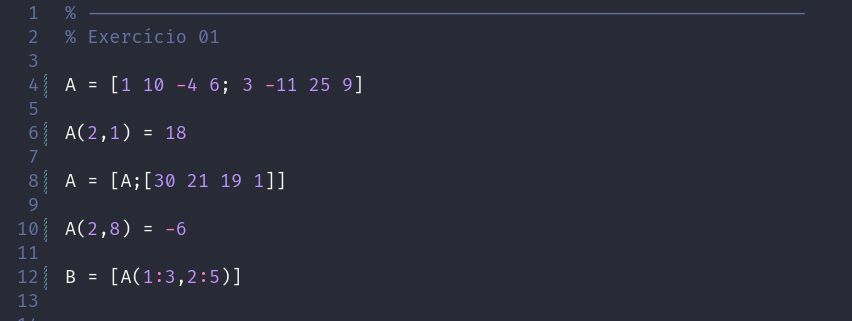
\includegraphics{01.png}
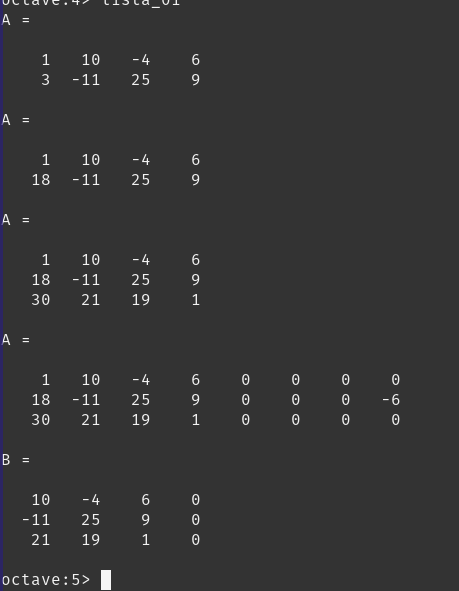
\includegraphics{01.1.png}

\newpage
\titulo{Exercício 02}
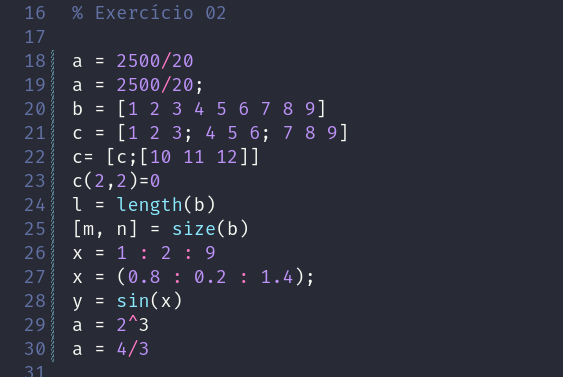
\includegraphics{02.png}
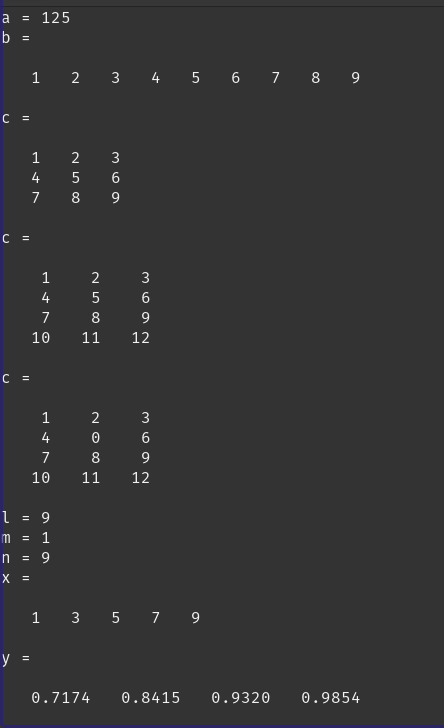
\includegraphics[scale=0.7]{02.1.png}
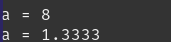
\includegraphics{02.2.png}

\newpage
\titulo{Exercício 03}
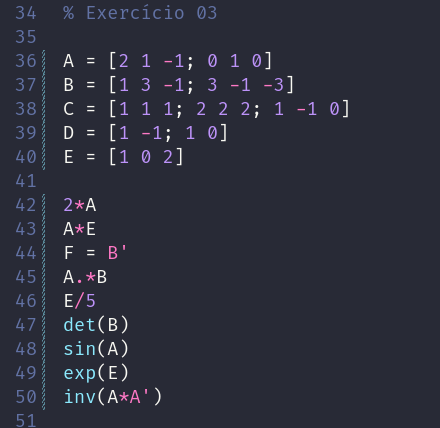
\includegraphics{03.png}


\newpage
\titulo{Exercício 04}
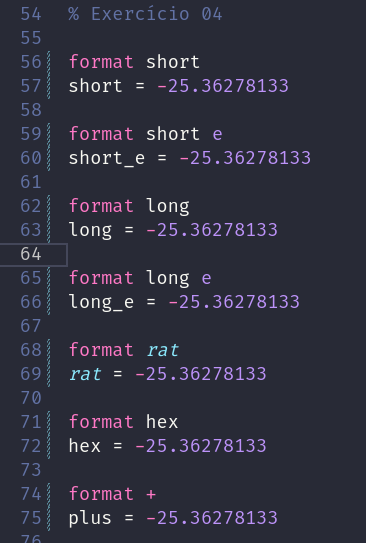
\includegraphics[scale=0.7]{04.png}
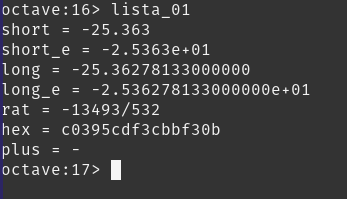
\includegraphics{04.1.png}

\newpage
\titulo{Exercício 05}
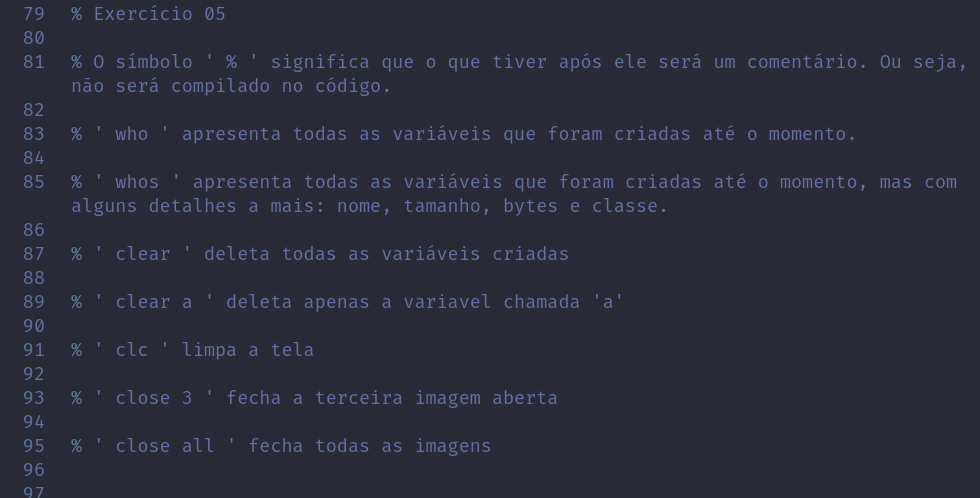
\includegraphics[scale=0.5]{05.png}

\newpage
\titulo{Exercício 06}
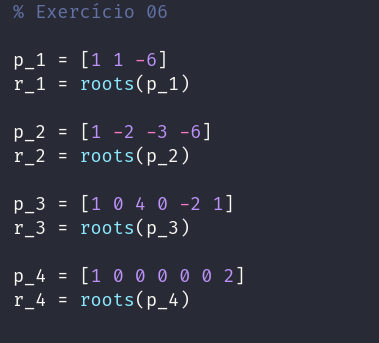
\includegraphics[scale=0.7]{06.png}
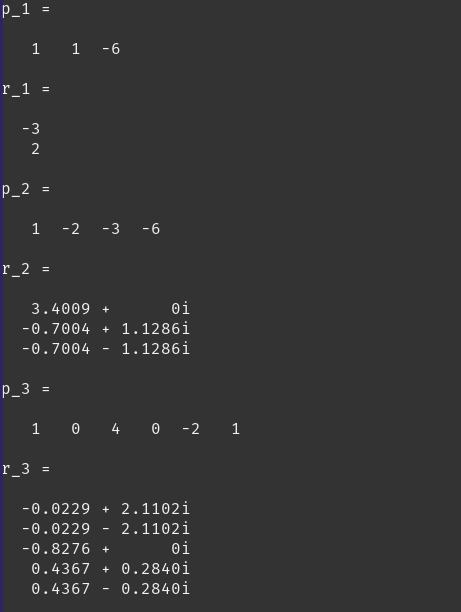
\includegraphics[scale=0.7]{06.1.png}
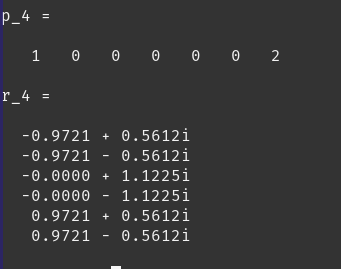
\includegraphics[scale=0.7]{06.2.png}

\newpage
\titulo{Exercício 07}
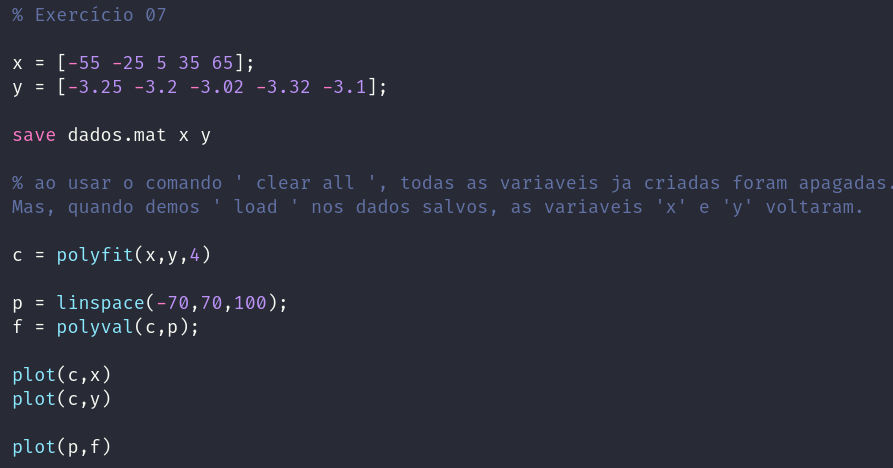
\includegraphics[scale=0.5]{07.png}
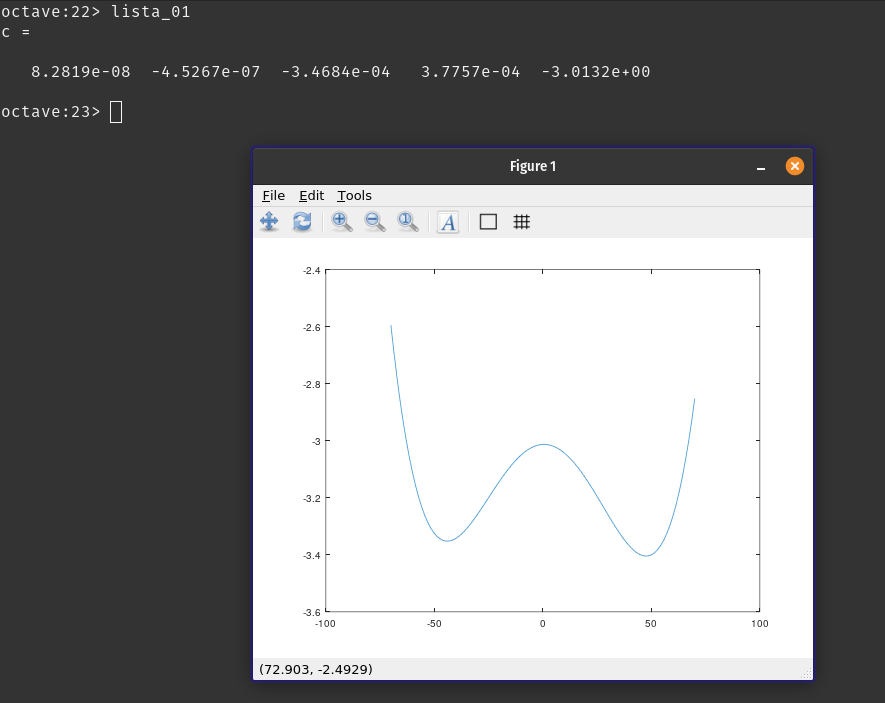
\includegraphics[scale=0.5]{07.2.png}

\newpage
\titulo{Exercício 08}
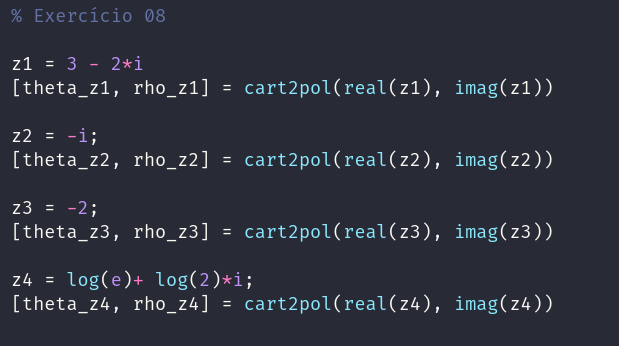
\includegraphics[scale=0.8]{08.png}

\newpage
\titulo{Exercício 09}
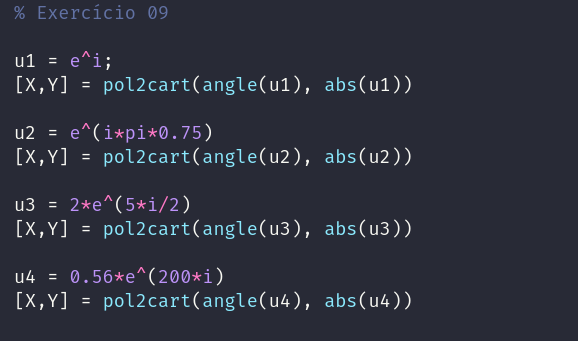
\includegraphics{09.png}
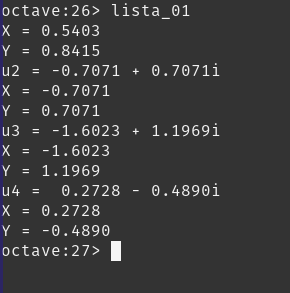
\includegraphics{09.1.png}

\newpage
\titulo{Exercício 10}
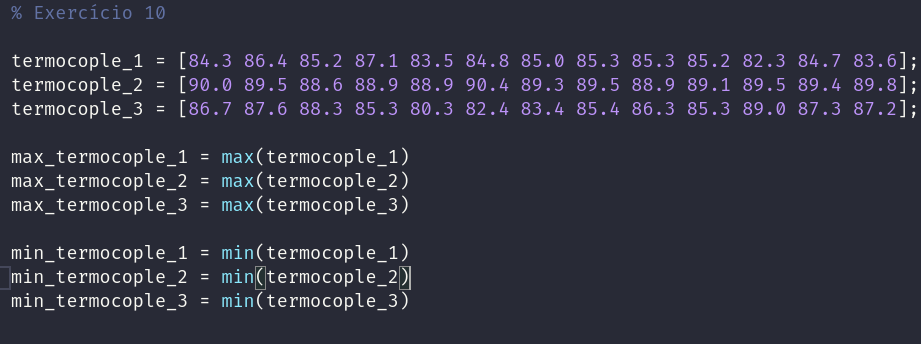
\includegraphics[scale=0.5]{10.png}
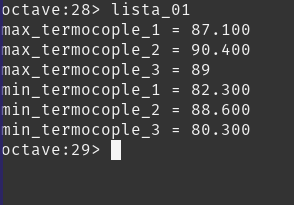
\includegraphics{10.1.png}

\newpage
\titulo{Exercício 11}
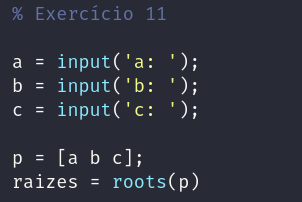
\includegraphics{11.png}
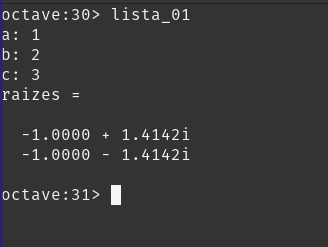
\includegraphics{11.1.png}

\newpage
\titulo{Exercício 12}
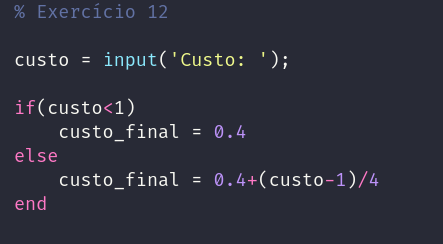
\includegraphics{12.png}
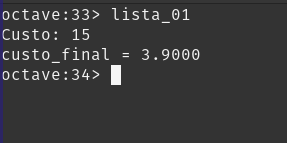
\includegraphics{12.1.png}

\newpage
\titulo{Exercício 13}
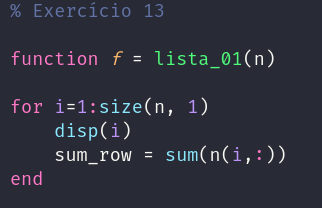
\includegraphics[scale=0.7]{13.png}
\newline
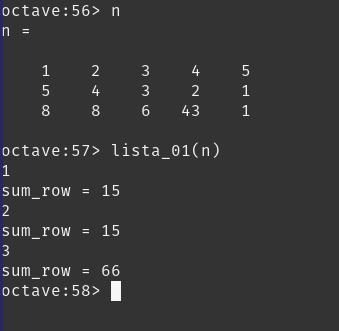
\includegraphics{13.1.png}

\newpage
\titulo{Exercício 14}
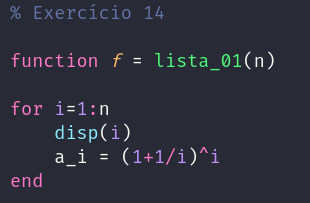
\includegraphics{14.png}
\newline
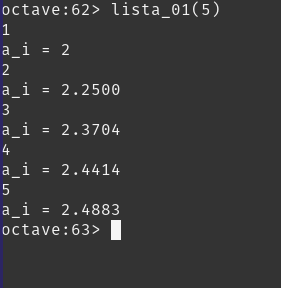
\includegraphics{14.1.png}

\newpage
\titulo{Exercício 15}
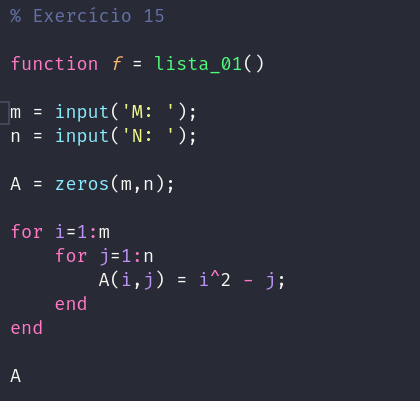
\includegraphics{15.png}
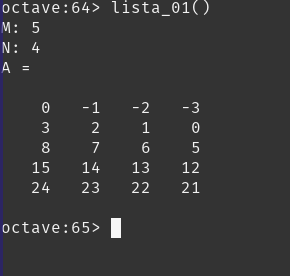
\includegraphics{15.1.png}

\newpage
\titulo{Exercício 16}
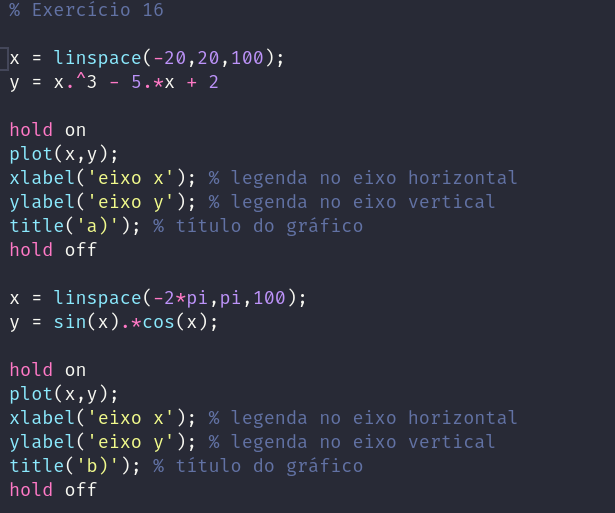
\includegraphics[scale=0.5]{16.png}
\newline
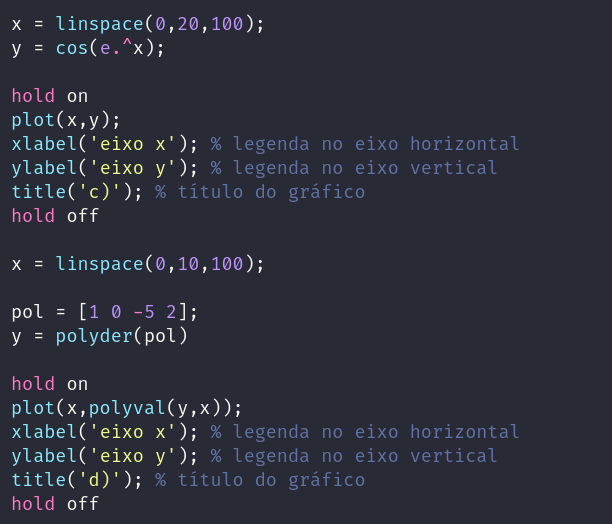
\includegraphics[scale=0.5]{16.1.png}
\newline
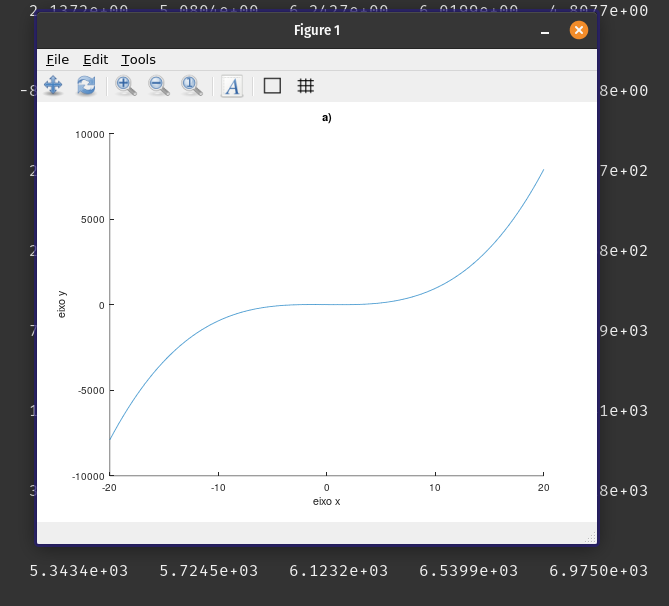
\includegraphics[scale=0.5]{16.2.png}
\newline
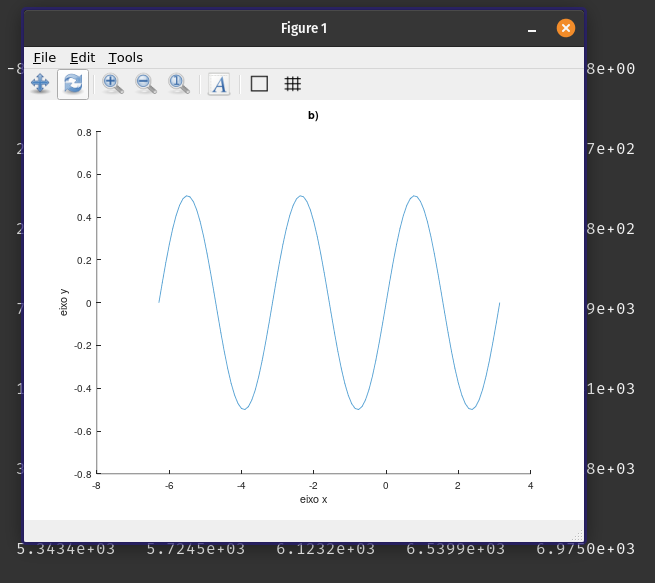
\includegraphics[scale=0.5]{16.3.png}
\newline
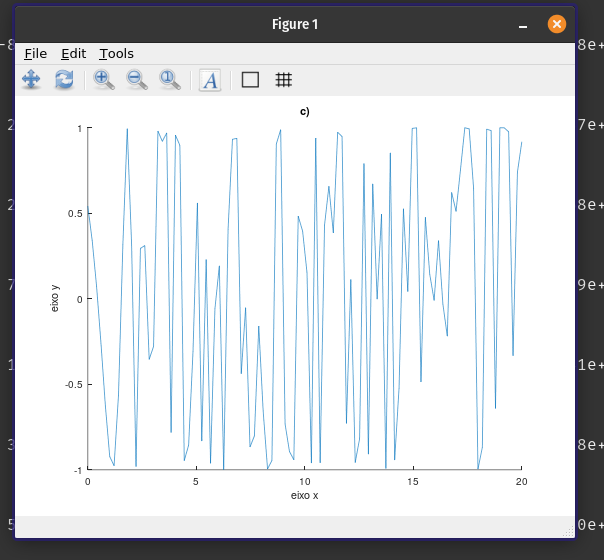
\includegraphics[scale=0.5]{16.4.png}
\newline
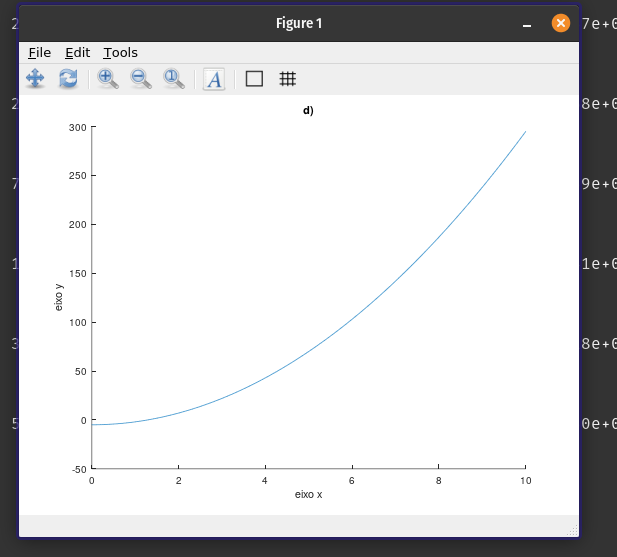
\includegraphics[scale=0.5]{16.5.png}

\newpage
\titulo{Exercício 17}
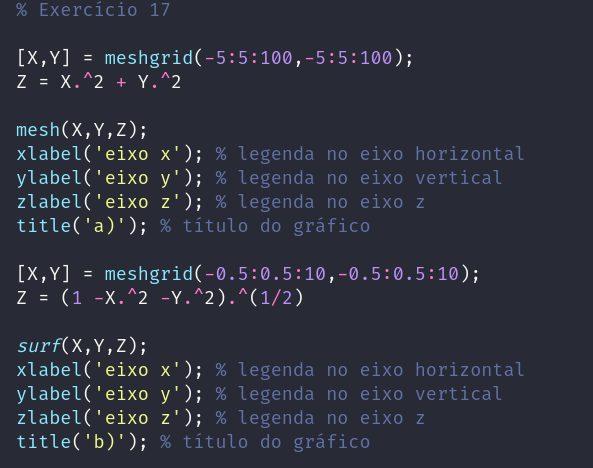
\includegraphics[scale=0.5]{17.png}
\newline
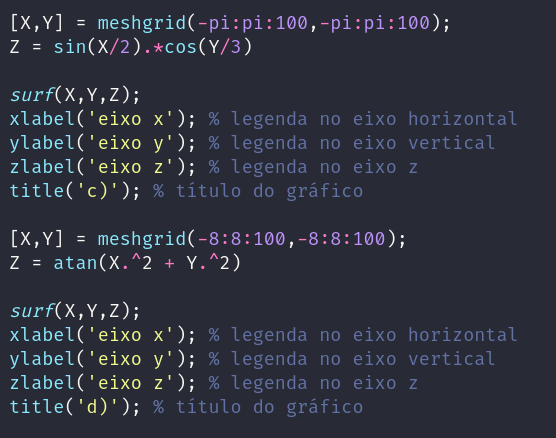
\includegraphics[scale=0.5]{17.1.png}
\newline
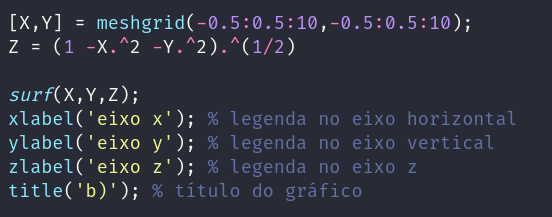
\includegraphics[scale=0.5]{17.3.png}
\newline
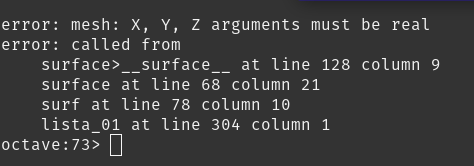
\includegraphics[scale=0.5]{17.4.png}
\newline
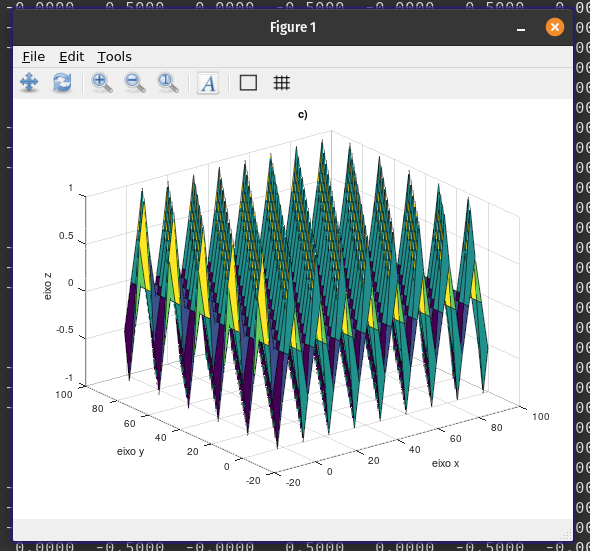
\includegraphics[scale=0.5]{17.5.png}
\newline
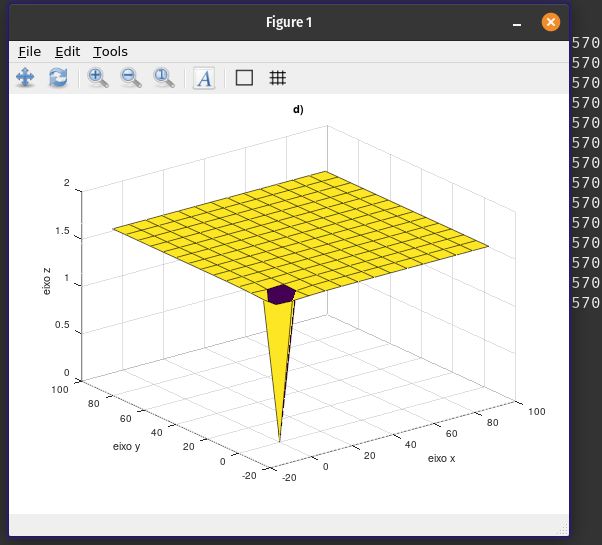
\includegraphics[scale=0.5]{17.6.png}
\newline

\newpage
\titulo{Exercício 18}
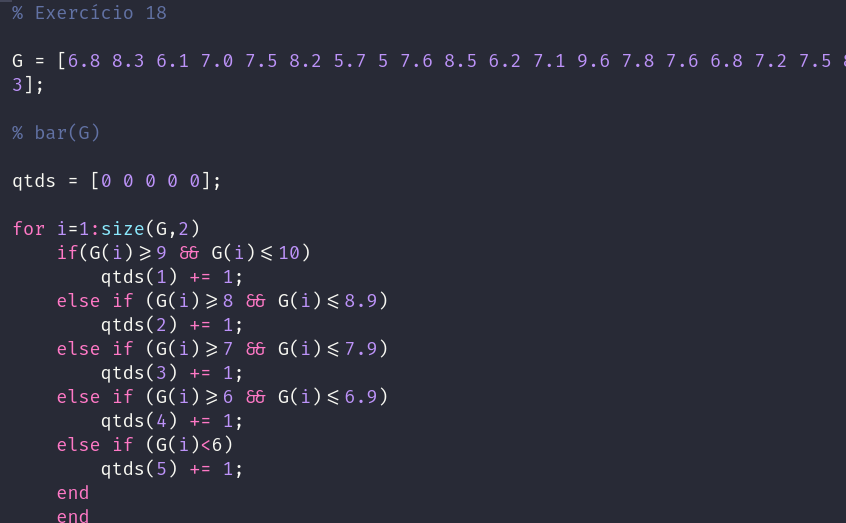
\includegraphics[scale=0.5]{18.png}
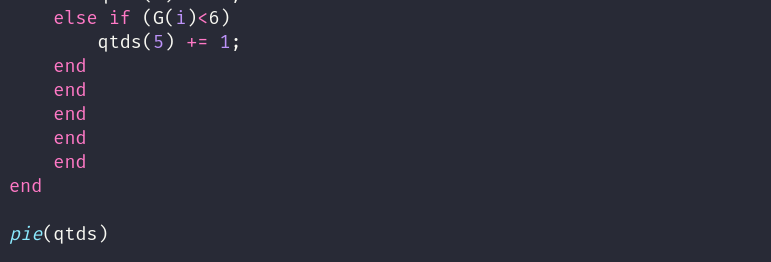
\includegraphics[scale=0.5]{18.1.png}
\newline
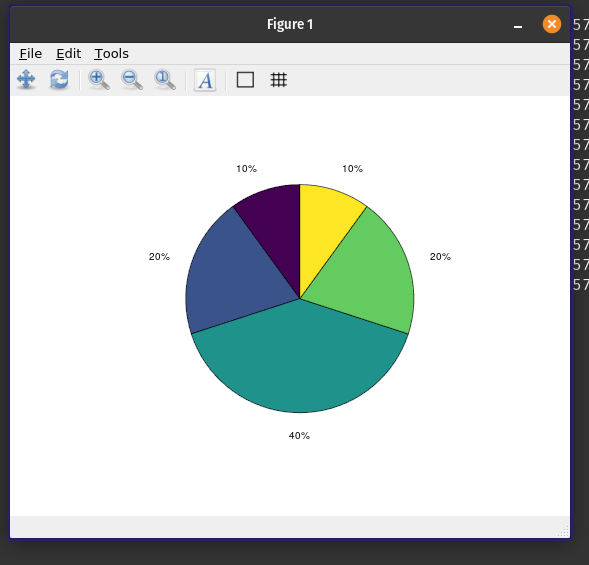
\includegraphics[scale=0.5]{18.2.png}

\newpage
\titulo{Exercício 19}
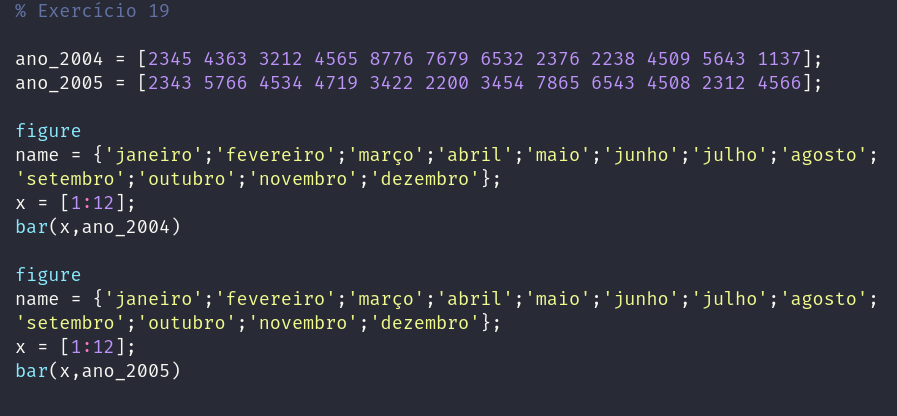
\includegraphics[scale=0.5]{19.png}
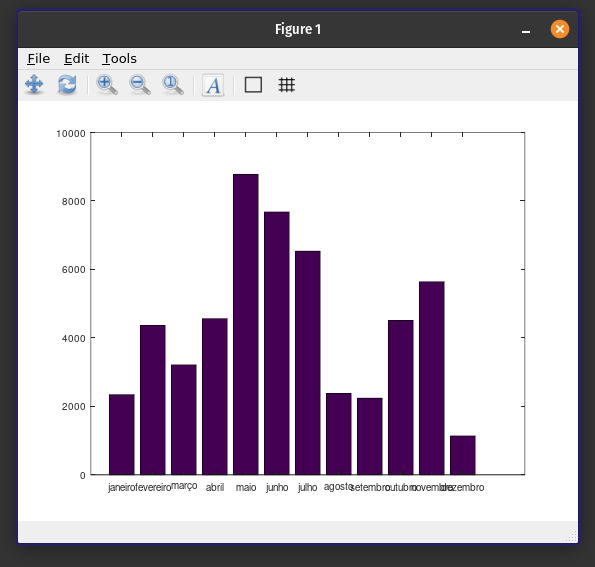
\includegraphics[scale=0.5]{19.1.png}
\newline
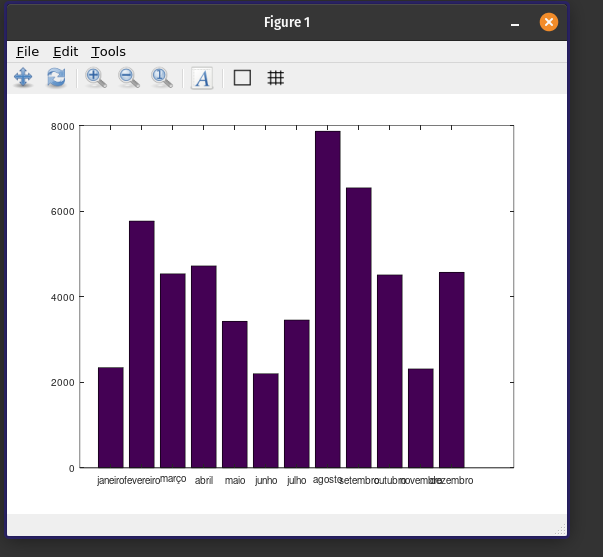
\includegraphics[scale=0.5]{19.2.png}


\newpage
\titulo{Exercício 20}
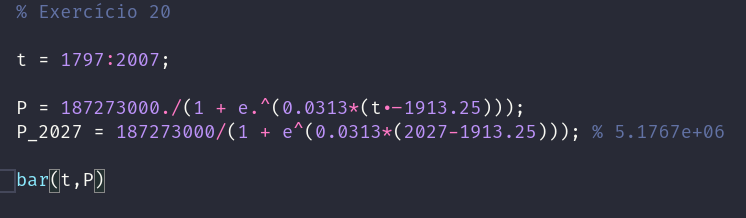
\includegraphics[scale=0.5]{20.png}
\newline
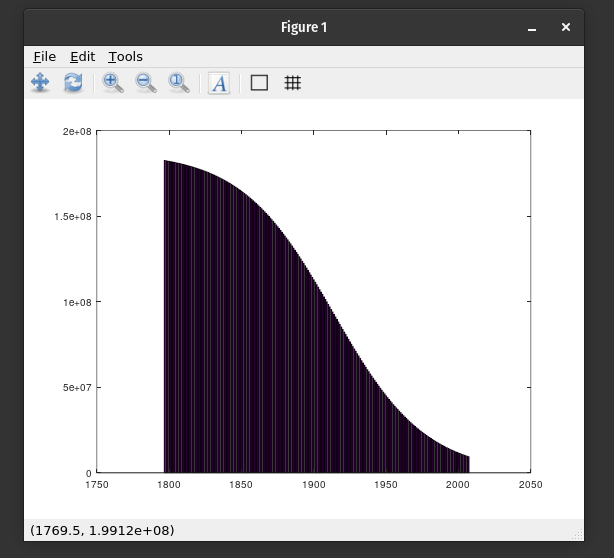
\includegraphics[scale=0.5]{20.1.png}





\end{document}
